%cel

\chapter{Wprowadzenie} \label{wstep}

Ultraszybkie lasery znajdują wiele zastosowań w przeróżnych dziedzinach - informatyka, fizyka, medycyna...  Dla przykładu, takie lasery są wykorzystywane w kryptografii kwantowej czy przy systemach telekomunikacji o szybkości 10\,Gb/s lub wyższej \cite{vecsel}. W przypadku kryptografii kwantowej wiązka z ultraszybkiego lasera jest "wstrzykiwana" do wiązki innego lasera, dzięki temu ograniczone są odchylenia sygnału od jego ustalonych charakterystyk (ang. time jitter) i pojawia się możliwość szybkiego przekazywania zaszyfrowanej informacji (z prędkością $1$\,Mb/s) \cite{quant}. Natomiast w przypadku systemów telekomunikacji, ultraszybkie lasery są używane ze względu na małą ilość zakłóceń w emitowanej wiązce w porównaniu do laserów ciągłych \cite{vecsel}.

Pierwsze ultrakrótkie impulsy, o długości rzędu pikosekund, w laserach na ciele stałym zostały wyemitowane dzięki pasywnie synchronizującym mody laserowi Nd:szkło, zaprojektowanemu przez De Marię i współpracowników w roku 1966, 6 lat po zaprezentowaniu pierwszego lasera w historii \cite{hist}. %Laser ten, jednak, posiadał jedną znaczącą wadę: uzyskany impuls jest modulacją amplitudy poszczególnych modów wiązki, a co za tym idzie impuls ten jest relatywnie długi.
Przełom w tworzeniu ultrakrótkich impulsów w laserach na ciele stałym nastał w 1991 roku razem z odkryciem samosynchronizacji modów w laserze Ti:szafir przez grupę Sibbett \cite{hist2}. To zjawisko jest dziś znane w literaturze jako synchronizacja metodą samoogniskowania Kerra (ang. Kerr lens mode locking - KLM) i polega ono na samonasyceniu się absorbenta, którym jest kryształ ośrodka czynnego. Dzięki KLM, praktycznie w każdym laserze na ciele stałym zachodzi samorzutna synchronizacja modów, a co za tym idzie generacja impulsów piko- i femtosekundowych bez potrzeby stosowanie urządzeń modulujących, gdyż modulatorem jest sam ośrodek czynny. Jednak, w celu osiągnięcia impulsów stabilnych, powtarzalnych i ze ściśle zdefiniowanym kształtem należy zastosować urządzenie kontrolujące dyspersję grupowego opóźnienia (ang. Group Delay Dispersion - GDD) \cite{hist3}, która to jest zdefiniowana jako druga pochodna zmiany fazy $\phi$ fali przechodzącej przez strukturę po częstotliwości $\omega$:
\begin{equation}
    GDD = \frac{d^2\phi}{d\omega^2},
\end{equation}
i charakteryzuje wpływ zjawiska dyspersji na czas przejścia przez strukturę. Im wartość GDD jest większa tym ten wpływ jest większy i fala jest opóźniana.

Dalszy rozwój laserów o ultrakrótkich impulsach opierał się na zaprojektowaniu tego urządzenia. W taki oto sposób pojawiły się zwierciadła ze zmiennymi grubościami warstw (ang. chirped mirrors) po raz pierwszy zaprezentowane przez grupę TU-Vienna, aby chwilę później być rozbudowane w ramach koncepcji zwierciadeł ze zmienną grubością pary warstw jak i zmienną względną grubością warstw w każdej parze (ang. double chirped mirror) przez ETH-Zurich \cite{hist2}.

Dalsze prace związane ze zwierciadłami DBR dotyczyły prób uzyskania jak najmniejszej i najstabilniejszej wartości dyspersji grupowego opóźnienia przy zachowaniu jak najwyższej odbijalności lustra. Pojawiły się prace próbujące rozwiązać sposób analitycznie, jak np. praca \cite{dbr3}, gdzie wyprowadzono następujące równanie pozwalające określić grubości warstw na podstawie żądanej wartości GDD:
\begin{equation}
    k_B(m)=k_B^{max}\cdot\sqrt{1-\frac{4\pi^2}{c^2D_0(\pi-|\kappa_0|)(k_B^{max})^2}|m|},
\end{equation}
gdzie: $k_B$ --- lokalny numer fali Bragg'a, zdefiniowany jako $k_B = \frac{\pi}{n_1d_{1,m}+n_2d_{2,m}}$, $k_B^{max}$ --- największy lokalny numer fali Bragg'a pozwalający otrzymać ujemne GDD, $m$ --- numer pary warstw (założono, że jest to wartość ciągła), $c$ --- szybkość światła w próżni, $D_0$ --- wartość bezwzględna żądanej wartości GDD oraz $\kappa_0$ --- współczynnik sprzężenia między warstwami w parze. \\
Z tak wyprowadzonego wzoru skorzystano w celu znalezienia struktury złożonej z półprzewodników o współczynnikach załamania kolejno $n_1 = 3,0$ i $n_2 = 3,5$. 
%Dla tych materiałów współczynnik sprężenia $\kappa_0 \approx -0,154$. 
Ustalono wartość bezwzględną żądanej wartości GDD aby wynosiła $D_0 = 1000\fs$. $k_B^{max}$ ustalono natomiast na wartość $2\pi/980\nm$. Tak zaprojektowane zwierciadło charakteryzuje się, faktycznie, wartością GDD na poziomie $-1000\fs$ przy dużej odbijalności, tak jak przedstawiono to na rysunku \ref{fig:anal}.

\begin{figure}[H]
    \centering
    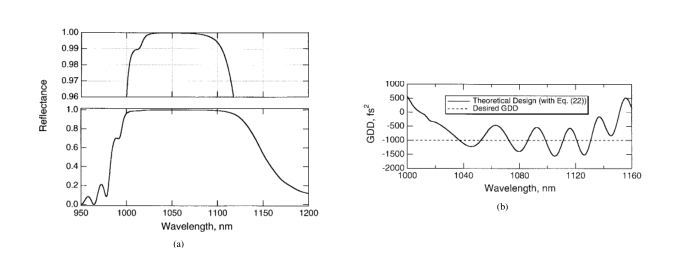
\includegraphics[width=\textwidth]{figures/anal.png}
    \caption[Współczynnik odbicia i GDD w przypadku rozwiązania analitycznego]{Współczynnik odbicia i GDD w przypadku rozwiązania analitycznego \cite{dbr3}}
    \label{fig:anal}
\end{figure}

Otrzymana wartość GDD jest niska, lecz nie jest do końca stabilna. Dlatego próbowano uzyskać jeszcze lepsze wartości tego parametru korzystając z innych podejść do problemu oraz z potęgi komputerów w celu zoptymalizowania obliczeń. W taki też sposób pojawiła się między innymi praca \cite{dbr2} wykorzystująca metodę macierzy przejścia, która jest szczegółowo omówiona w 3.1, w celu wyznaczenia wzorów pozwalających obliczyć współczynnik odbicia i GDD dla danego zwierciadła. Ponadto tę metodę zoptymalizowano korzystając z algorytmów genetycznych aby uzyskać jak najlepsze wyniki. Udało się wyznaczyć strukturę z wartością GDD wynoszącą około $-3600\fs$ przy zakresie długości fali $1030 - 1050\nm$. Metoda ta okazała się skuteczna, lecz wyniki wciąż można próbować polepszyć. Jedną z rzeczy, która jeszcze nie została zrobiona jest sprawdzenie efektu zastosowania innego rodzaju algorytmów, m.in. algorytmów rojowych, należących do grupy algorytmów stadnych.

Dlatego też niniejsza praca przedstawia próbę otrzymania jeszcze lepszych wyników wykorzystując optymalizację obliczeń przy wykorzystaniu algorytmów rojowych. Dodatkowym celem pracy było poznanie sposobu działania tych właśnie algorytmów i sprawdzenie ich potencjału przy rozwiązywaniu podobnych problemów.